\documentclass[12pt, spanish]{article}
\usepackage[spanish]{babel}
\selectlanguage{spanish}
\usepackage{natbib}
\usepackage{url}
\usepackage[utf8x]{inputenc}
\usepackage{graphicx}
\graphicspath{{images/}}
\usepackage{array}
\usepackage{float}
\usepackage{siunitx}
\usepackage[table,xcdraw,dvipsnames]{xcolor}
\usepackage{longtable}
\usepackage{parskip}
\usepackage{fancyhdr}
\usepackage{vmargin}
\usepackage{listings}
\usepackage{adjustbox}
\usepackage{subfig}
\usepackage{minted}
\usepackage[shortlabels]{enumitem}
\setlist[enumerate]{
labelsep=8pt,
labelindent=0.3\parindent,
itemindent=0pt,
leftmargin=*,
before=\setlength{\listparindent}{-\leftmargin},
}

\def\code#1{\texttt{#1}}
\usepackage[default]{sourcesanspro}
\usepackage{tcolorbox}
\usepackage{etoolbox}
\BeforeBeginEnvironment{minted}{\begin{tcolorbox}}%
\AfterEndEnvironment{minted}{\end{tcolorbox}}%

\setmarginsrb{2 cm}{1 cm}{2 cm}{2 cm}{1 cm}{1.5 cm}{1 cm}{1.5 cm}

\title{Práctica 2: Agentes Reactivos/Deliberativos \hspace{0.05cm} }
\date{}
\author{
Yeray López Ramírez \\
}

\renewcommand*\contentsname{hola}

\makeatletter
\let\thetitle\@title
\let\theauthor\@author
\let\thedate\@date
\makeatother

\pagestyle{fancy}
\fancyhf{}
\rhead{}
\chead{\thedate}
\lhead{\thetitle}
\cfoot{\thepage}

\begin{document}
%%%%%%%%%%%%%%%%%%%%%%%%%%%%%%%%%%%%%%%%%%%%%%%%%%%%%%%%%%%%%%%%%%%%%%%%%%%%%%%%%%%%%%%%%
\begin{titlepage}
  \centering
  \vspace*{0.5 cm}
  
\includegraphics[scale = 0.50]{ugr.png}\\[1.0 cm]
  %\textsc{\LARGE Universidad de Granada}\\[2.0 cm]   
  \textsc{\huge Grado en Ingeniería Informática}\\[0.5 cm]
  \rule{\linewidth}{0.2 mm} \\[0.4 cm]
  { \huge \bfseries \thetitle}\\
  \rule{\linewidth}{0.2 mm} \\[1.5 cm]
  
  \begin{minipage}{0.4\textwidth}
    \begin{flushleft} \large
        \emph{Autor:}\\

        \theauthor
        \end{flushleft}
        \end{minipage}~
        \begin{minipage}{0.4\textwidth}
        \begin{flushright} \large
        \emph{Curso:2ºC \\
        Asignatura: Inteligencia Artificial \\
        Fecha: 16 de Mayo de 2022
        }
    \end{flushright}
\end{minipage}\\[1 cm]


\vfill
  
\end{titlepage}

\newpage

%%%%%%%%%%%%%%%%%%%%%%%%%%%%%%%%%%%%%%%%%%%%%%%%%%%%%%%%%%%%%%%%%%%%%%%%%%%%%%%%%%%%%%%%%


\tableofcontents
\pagebreak

%%%%%%%%%%%%%%%%%%%%%%%%%%%%%%%%%%%%%%%%%%%%%%%%%%%%%%%%%%%%%%%%%%%%%%%%%%%%%%%%%%%%%%%%%

\section{Objetivo de la Práctica}
En esta práctica, al igual que la anterior, se nos presenta a un agente que se sitúa en un mundo de BelKan con 4 niveles diferentes. Mi objetivo principal es conseguir que el agente supere los niveles antes de agotar los ciclos de ejecución. Por ello describiré el comportamiento general de mi agente y lo desarrollaré después.

\section{Comportamiento general}
El agente que he diseñado consta de 3 fases: Chequear, planear y ejecutar. Se explica detalladamente en los siguientes párrafos:
\begin{enumerate}
 \item En su primera fase comprueba su estado previo y actual. A partir de esa información actualiza el mapa, su posición y orientación ademas de establecer los objetivos, visionar el mapa y establecer las zonas de Peligro(explicadas adelante). Siempre entra en esta fase.

 \item En su segunda fase toma un plan según el nuvel en el que se encuentre. Para los niveles 0,1 y 2 solo comprueba que no tenga nada planeado y ejecuta el pathFinding.


  \item En su tercera fase ejecuta las acciones guardadas en la lista de acciones ``Plan''. Se guarda la primera accion del plan y se elimina de la lista. Siempre que el plan NO esté vacío, ignorará la fase 2 y entrará directamente en esta fase hasta finalizarla.

\end{enumerate}


\section{Comportaiento Avanzado: PathFinding}
En la siguiente sección hablaremos sobre los pathFinding:

\subsection{pathFindingProfundidad}
Este algoritmo es el más sencillo de todos y nos sirve de prueba inicialmente para entender el funcionamiento de la nueva práctica. Su eficiencia es horrible y su desempeño aún más.

\subsection{pathFindingAnchura}
Este algoritmo es literalmente igual que el anterior a diferencia de que usa una cola en vez de una pila. Tras aprovechar el algoritmo de anchura y hacer la correspodiente modificación vemos que efectivamente funciona pero es terriblemente lento. Así que para mejorar eso he añadido poda al árbol a través del set frontera. Este set ordena los nodos de menor a mayor pasos y poda los nodos que ya están en nuestra secuencia solución. Esto aumenta enormemente su eficiencia y hace el algoritmo manejable incluso en grandes distancias.

\subsection{pathFindingCosteUniforme}
Por último tenemos al coste uniforme cuya implementación se ha basado en el pseudocódigo de la teoría del Tema 3.

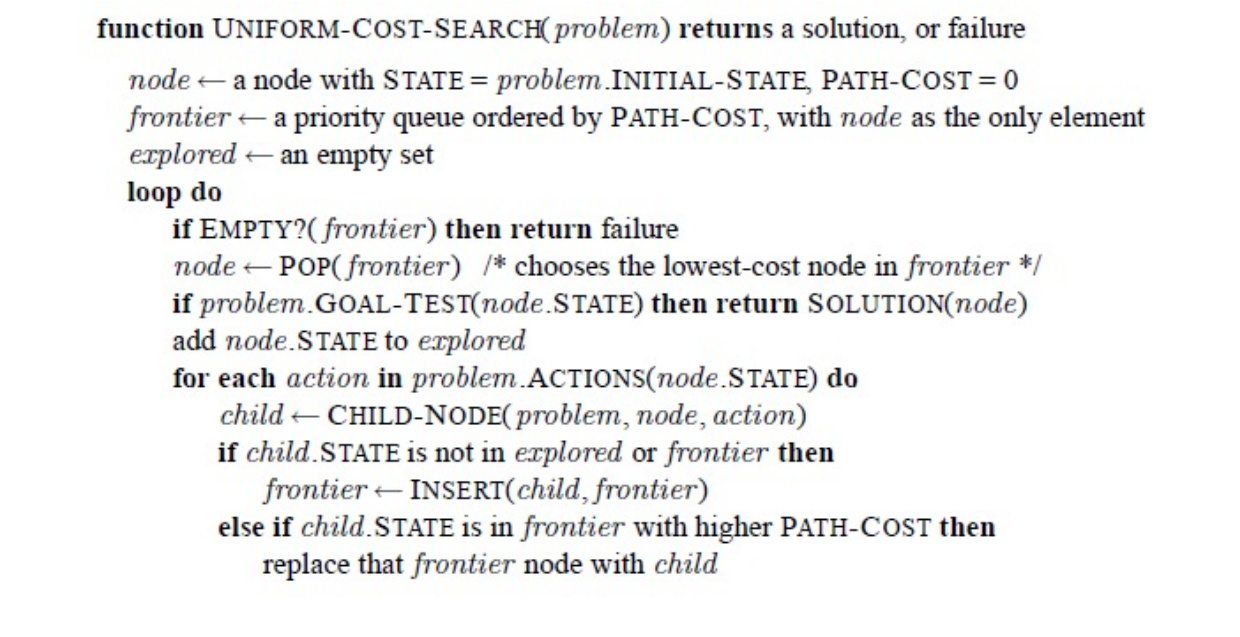
\includegraphics[scale = 0.50]{costeUniforme.png}

Para su funcionamiento usamos una cola de prioridad que ordena los nodos según su coste usando una función calcularCoste, que es una interpretación de las tables de coste del guión. Al igual que en Anchura, aplicamos poda con frontera y modificamos los nodos con aquellos que tengan mejor coste. Este algoritmo es el más rápido con diferencia y es el que usaré de forma indiferente para el nivel 3 y 4

\subsection{Nivel 3}
Para este nivel se nos pide explorar el máximo mapa posible al más puro estilo de la práctica 1 con la diferencia de que disponemos de algoritmos que nos van a facilitar la vida increiblemente.
En mi caso, he utilizado una modificación del coste Uniforme que busca las casillas sin explorar más cercanas. Se podan los nodos de Bosque y Agua que no posean objetos cerca para aumentar su eficiencia.

\subsection{Nivel 4}
Para este nivel se nos pide ir a por la mayor cantidad de objetivos posible. Para ello he utilizado también el coste uniforme, en este caso no lo he modificado en absoluto. Para poder hacer uso del algoritmo correctamente he implementado las ``zonas de peligro`` que resumidamente son zonas adyacentes a aldeanos y lobos que son potencialmente peligrosas. Si el coste Uniforme se topa con una casilla Peligrosa, la poda y pasa a otra. La gestión de choques y empujones se ha abordado aplicando actWHEREIS cuando se activa el sensor de choque.


\vspace{5cm}
 \bibliographystyle{plain}
 \bibliography{biblist}


\end{document}
